\chapter{Background and Literature Review}

\epigraphhead[50]{\epigraph{\large{`The brain computes!'}}{Biophysics of Computation\\
by Christof Koch}}

\section{Scope of this Review}
This literature review provides a high level overview of the core topics relating to this dissertation, and provides context for the requirements and assumptions of the software development involved in this project. 

If one were to consider a brain as analogous to a computer, with the memories of
the brain as the hard drive, it is these memories that an  emulation of a brain
would require to be considered a continuation of a being
\autocite{eichenbaum_cognitive_2011}. The academic schools that study and debate
the inner workings and logistics of the human mind are many in number, and it is
outside the scope of this project to summarise all of them in detail.  This
literature review is therefore concerned with the replication of the neural
structure and its constituent function at a low level.

% TODO: Levels of emulation pg.13 Bostrom and Sandburg Roadmap

\section{Spiking Neural Networks}

\begin{quote}
    `The brain computes! This is accepted as a truism by the majority
    of neuroscientists engaged in discovering the principles employed in the
    design and operation of nervous systems. What is meant here is that any
    brain takes the incoming sensory data, encodes them into various biophysical
    variables, such as the membrane potential or neuronal firing rates, and
    subsequently performs a very large number of illspecified operations,
    frequently termed computations, on these variables to extract relevant
    features from the input.'
    \begin{flushright}
        \textit{-- Christof Koch \\ Biophysics of Computation}
    \end{flushright}
\end{quote}

The mammalian nervous system is principally composed of neurons and glial cells.
Glial cells primarily perform supplementary roles in the function and processing
of data in the nervous system, but it is still not fully understood what further
role they play \autocite{walz_role_1989}. Neurons are less numerous in the
nervous system, and are chemically unique in their functioning in the body.

\begin{figure}[t]
    \centering
    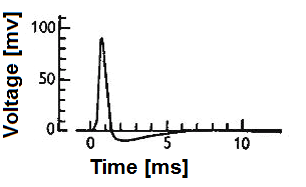
\includegraphics{figures/graphs/huxhog_spike.png}
    \DoubleCaption{The typical form of a neuronal action potential}
    {\small{Created by Nir.nossenson@wikipedia.com, licenced 
            \href{https://creativecommons.org/licenses/by-sa/4.0/deed.en}{CC BY-SA 4.0}}}
    \label{neuronalactionpotentialexample}
\end{figure}
\vspace{1ex}

Each neuron acts as a gate of sorts, holding or releasing its potential in
response to signals as part of a greater network of neurons. This release often
takes the form of a spike, as seen in figure \ref{neuronalactionpotentialexample}.
Together, the neurons in these networks perform the signal processing and
routing that "computes" the many sensory inputs to the nervous system
\autocite{koch_biophysics_2004}. While not all neurons are spiking neurons, it
is the properties of spiking neurons and the interactions between them that are
the focus of this review and ultimately this document.

\subsection{Hodgkin–Huxley model}

In 1952, Alan Hodgkin and Andrew Huxley described a model of the squid giant
axon that accurately reflects the both the chemical changes and the form of the
action potential spike in the axon. \autocite{hodgkin_quantitative_1952}

The strength of the Hodgkin–Huxley model is in its adaptability. Every change in
a neuron during a spike, be it chemical or physical, can be mapped across, and
more complex behaviour can be recreated in the model thanks to its basis in the
core chemistry of a neuron. However, this complexity is not without pitfalls as
the computational power required to simulate such advanced models is so large,  that it is no longer feasible to simulate in a network.

\subsection{Faster neuron models for large scale computation}

While it can be desirable to accurately model and simulate the chemical
interactions between individual components of the nervous system, it is
computationally infeasible to do so on a scale similar to that of a real-world
system due to the computational complexity of the Hodgkin - Huxley equations.
Fortunately, as a network becomes larger, the exact mechanisms of its individual
components can be approximated, and faster activation or threshold functions
that perform similarly to real ones can be substituted.

One such example of a simple model of a spiking neuron is the Leaky Integrate
and Fire (LIF) neuron. It uses a simple threshold function to approximate the
action potential spike generation of a Hodgkin–Huxley neuron
\autocite{trappenberg_fundamentals_2009}. As this is a relatively simple
approximation, it is tempting to assume that such a model would prove inaccurate
for anything more than basic prototypes, however LIF models have been shown to
replicate spiking patterns of more complex models with a low margin of error,
provided the models are under natural conditions
\autocite{teeter_generalized_2018}. This document will go into more detail on
the equations and implementation of LIF neurons in Chapter 3, starting with
equation \eqref{eq:LIF_TC}.


\section{Computational models for brain simulation}

The coupled differential equations that define a compartmental model of a neuron
can be solved numerically, and can therefore be programmed in a high-level
programming language relatively simply. However, while programmatically solving
differential equations is straightforward in principle, the computational power
and provision of memory required makes simulating large networks of neurons
difficult to do in practice \autocite{trappenberg_fundamentals_2009}. Existing
simulation packages provide a foundation from which biological experiments can
be conducted, and aim to abstract away purely computational concerns. Some of
these packages that have different approaches to solving this are described in
more detail below.

\subsection{Representing time in neural simulations}

There are several approaches that can be taken with respect to both simulating
individual neuron activity, and more general network activity. On the level of
individual components of a simulated network, the two predominant choices are
between a clock driven model and an event driven model. In a clock driven model,
continuous time is split into discrete chunks, and it is the size of these
chunks that determine the accuracy of the differential equations that define
neuronal behaviour. Conversely, an event driven model is asynchronous in nature,
where events such as spikes or learning updates that propagate backwards will
trigger further updates across the network. The advantage of a clock driven
model is its flexibility in using any differential equation, however, more
complex neuron models require a smaller time step leading to large computation
times. An event driven model, by comparison, computes in real time and spikes
are therefore unaffected by rounding errors from discretization
\autocite{brette_simulation_2007}. It is also possible to simulate population
dynamics to describe the average activity of neuronal populations
\autocite{trappenberg_fundamentals_2009}, which is ideal for modelling neuronal
populations that are on the scale of actual nervous systems with modern
computational power. The downside to this, however, is that such generalised
models are not always faithful approximations of true network effects between
neurons.

\subsection{Available neural simulation and modelling software packages}

\subsubsection{VERTEX}
The Virtual Electrode Recording Tool for EXtracellular potentials (VERTEX) is a
simulator for large networks of neurons written in the MATLAB programming
language. More specifically, it aims to reproduce the measurements that are
produced by in-vivo recordings from patients fitted with multi-electrode
arrays. This is achieved by locating each neuron in 3D space, placing virtual
electrodes in the same space, and calculating the change in potential at each
stage of the simulation at each electrode. The neuron model used in VERTEX is
also more advanced than similar models described in this section in that the
local field potential (LFP) of the neuron is spatially realistic
\autocite{tomsett_virtual_2015}. A major advantage of this design is that it
becomes easy to map between general neuronal activity in a simulated model and
brain activity of, say, a real-world patient in a medical trial.

A 2019 update to VERTEX introduced a range of simulation features, the most
notable of which for the purposes of this project is Spike Time Dependent
Plasticity (STDP), which dynamically adapts the weighting of synapses based on
the observed causality of pre-synaptic spikes on post-synaptic spikes
\autocite{thornton_virtual_2019}. Details on how this may be implemented and
used are covered further in Chapter 3. % TODO ref

VERTEX itself is multithreaded, and makes use of the compute pooling feature in
MATLAB to separate groups of tasks into separate logical threads. This means
that, with a sufficiently large model, doubling the number of available workers
in the pool nearly halves the time taken to simulate, as shown in figure
\ref{VERTEXparallel} below.

\begin{figure}[h!]
    \centering
    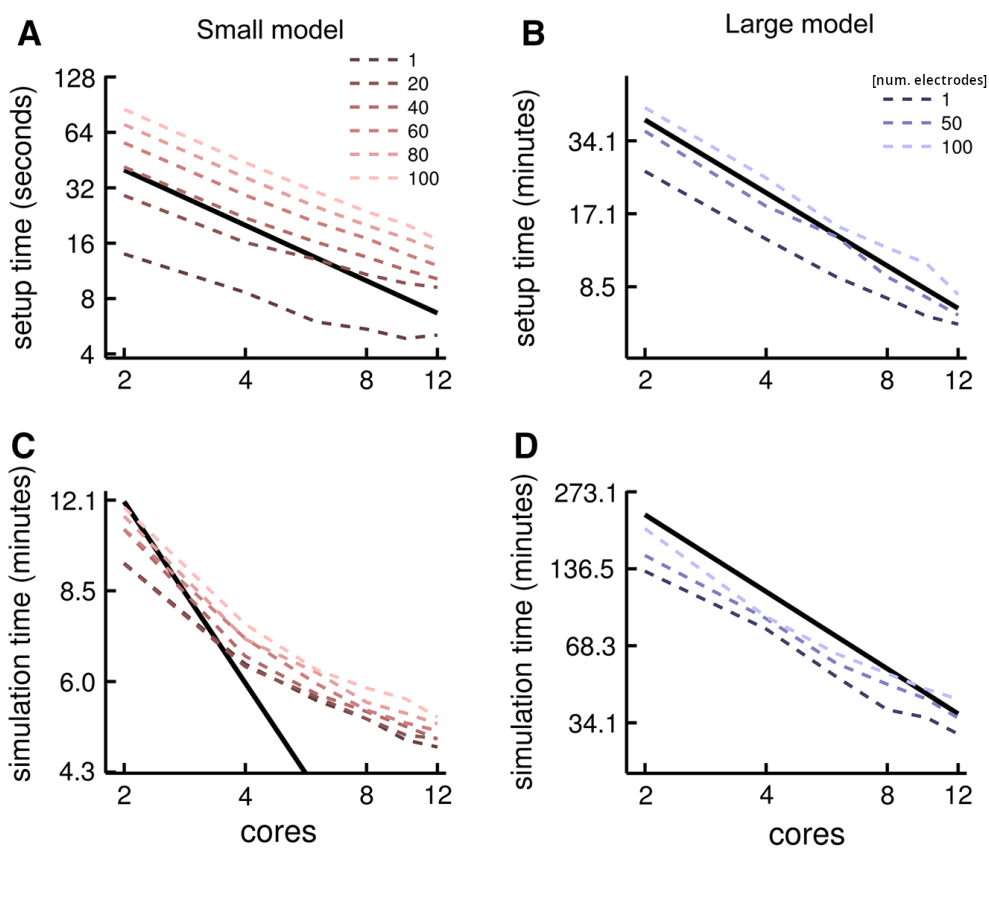
\includegraphics{figures/graphs/coresVERTEX.png}
    \caption[Impact of parallel computation on
        simulation performance in VERTEX] {Impact of parallel computation on
        simulation performance in VERTEX. Doubling the number of cores available
        for computation roughly halves the time taken to setup and run the
        simulation. Smaller models benefit less as fewer tasks can be
        independently shared across cores. \small{Reproduced from \cite{tomsett_virtual_2015}}}
    \label{VERTEXparallel}
\end{figure}
\vspace{1ex}

\FloatBarrier

\subsubsection{NEURON}

NEURON describes itself as ``a tool designed specifically for solving the
equations that describe nerve cells'' and provides a holistic environment for
developing and simulating models of individual neurons and neural networks. It
is particularly adept at modelling complex chemistry in neuron models, and can
be used when the field potential of a location very close to a neuron needs to
be accurately modelled \autocite{carnevale_neuron_2006}. This does, however,
mean that simulating large networks is computationally expensive, and more
complex models require correctly tuned parameters for each new feature which
increases the time setting up simulations.

Further simulation toolkits may be built atop NEURON, and one such example is
LFPy. LFPy is a Python tool using NEURON that aims to accurately provide
extracellular potential readings for single neuron models
\autocite{hagen_hybrid_2016}. It can also provide extracellular potential
readings for networks in the most recent versions \autocite{hagen_lfpy_2019},
however the caveat that NEURON based networks are limited in size by available
resources still holds.

\subsubsection{Brian}

"Brian" is another simulator for spiking neural networks, distributed as a
Python library. Brian offers a unique programming interface whereby the
differential equations that define a neuron can be written in plain-text and are
interpreted at runtime. Provided the equation can be interpreted correctly, this
approach makes computing mathematical models extremely simple, and is ideal for
quickly testing variations of a model \autocite{stimberg_brian_2019}. This is,
however, less useful for more complex relationships between neurons where the
plain-text mathematical syntax effectively develops its own API on top of the
Python API. Fortunately users of the library may provide native Python functions
to define the behaviour of their neurons if desired
\autocite{noauthor_functions_2020}. Neurons can be placed in physical space if
desired, but this is optional, and the complexity of actual neurons in a Brian
simulation is as complex as a programmer intends them to be. As a result, the
time taken to simulate a network is largely dependant on the time complexity of
the user-defined equations that define the neurons.

\subsection{Similarities in existing software packages}

Each of the software packages described above is capable of simulating a
network of neurons, but each has a distinct set of goals. Some, like Brian, are
intended as tools to study the spiking patterns and features of generic neural
networks, while VERTEX provides a more specialised tool that is optimised for
measuring the observed potential changes in a similar manner to capturing
experimental data. These differences are also seen in the API available to
developers
and the distribution methods that each package uses. VERTEX requires that the
user defines the parameters for neuron grouping and placement while abstracting
away the exact definition of the neuron behaviour, while NEURON and Brian are focussed on the neuron definition, and space placement or recording
mechanisms are functions largely left to the programmer to define.
\section{Imaging and Image Processing}

Considering prediction of brain activity requires that we look not only at the
current state of brain simulation, but also towards the future. A biological
brain processing the life of an organism, and a simulation of the same requires
that a link is made between the two: the state of the brain must be copied over as a
snapshot. This imaging process would likely take the form of an in vitro scan of
a preserved nervous system or some form of in vivo scan. These images would be
processed and turned into a model that could be simulated. Current techniques for imaging the brain give us some insight into to how this
uploading process might function and perform.

\subsection{Current Methods of Scanning the brain}

Given a 2D substrate such as a layer of brain tissue, there are several methods
of producing a high resolution image. These methods must balance the resolution
and noise levels required of model creation, with the speed with which the image
is taken \autocite{bostrom_whole_2008,mikula_progress_2016}.

\begin{figure}[h]
    \centering
    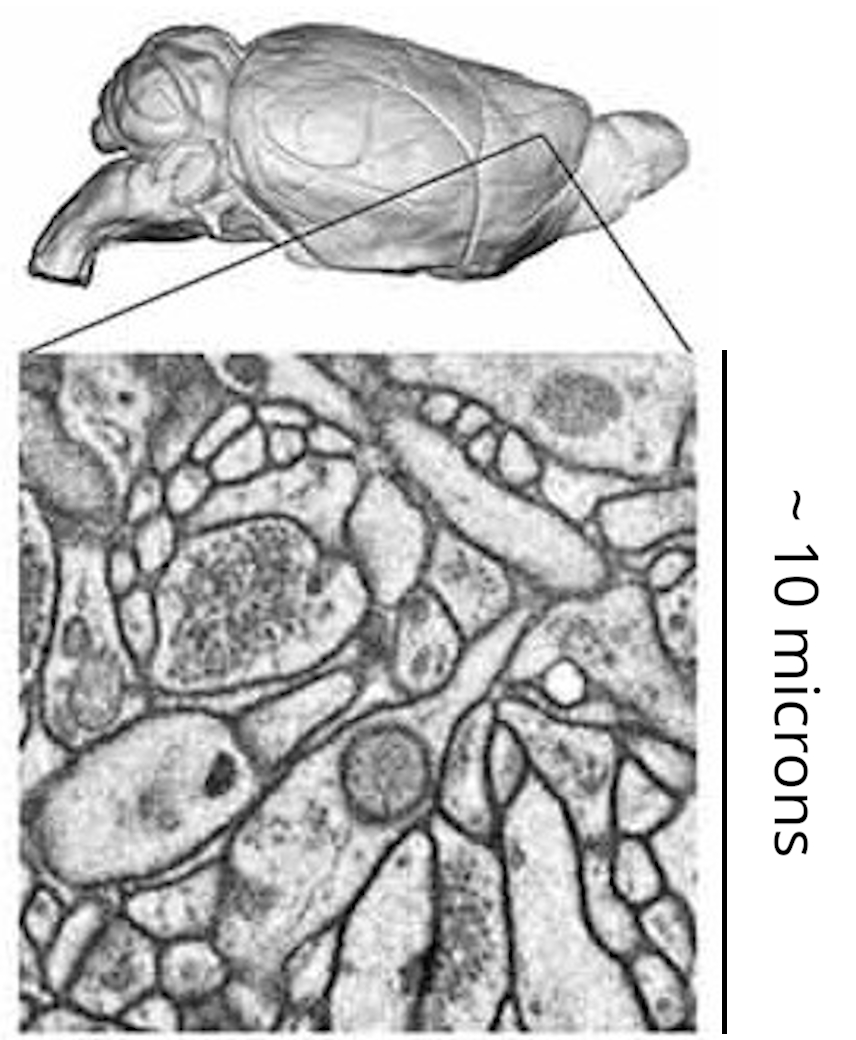
\includegraphics[scale=2]{figures/images/enlarge.jpg}
    \caption[Illustration of the scale of neurons in the brain of an adult mouse.]
    {Illustration of the scale of neurons in the brain of an adult mouse. While a mouse brain stores 1000 times fewer "byte" equivalents of information than a human, the size of neurons themselves is comparable. At the scale shown, the size and positions of neurons can be observed, but the exact morphology of the synapses between cannot be discerned. Adapted from \autocite[fig. 1]{mikula_progress_2016}}
    \label{scaleexample}
\end{figure}
\vspace{1ex}

Given the level of emulation that is intended from a model, the images that
synthesise the model must resolve a minimum level of detail. In figure
\ref{scaleexample}, the general position of neuron somas 
% what be somas
and the rough links between them can be identified, but more subtle morphologies
of these links are missing. Perhaps another imaging method could resolve further
detail. The specifications and drawbacks of several imaging methods are
described below.

\subsubsection*{MRI}

Magnetic Resonance Imaging (MRI) scanning is a common medical procedure, and can
be used to provide information about the regions of the brain and general
connective patterns between these regions. However, at current generally
available resolutions, MRI is not suitable for reconstructing any kind of neural
model that contains information pertaining to discrete connections between
neurons. Future technologies that enable brain emulation of the
biologically alive would need to offer a similar feature set as MRI scanning
whilst producing images many thousands of times more detailed. Such MRI
microscopy does exist currently, but is significantly more limited in scale,
scanning small chunks of cortical tissue at a very high resolution
\autocite{johnson_three-dimensional_1987,bostrom_whole_2008}.

\subsubsection*{Electron Microscope Scanning}

Electron Microscopy (EM) is a commonly used technology in any discipline where
one may wish to resolve detail at the scale of nano-metres. Since the wavelength
of accelerated electrons is much shorter than the wavelength of visible light,
the resolution of EM is not limited by diffraction in the same way as optical
imaging. As a result, it is the imaging method of choice for neural and cortical
tissue \autocite{marc_retinal_2013, kaynig_large-scale_2015}. EM is not without
drawbacks however, as brain tissue must be chemically preserved before
processing, making it a complicated and expensive procedure. 

One variation of EM is Correlative Light-Electron Microscopy (CLEM) which takes
a hybrid approach to imaging the brain with both optical and electron imaging.
CLEM therefore has the advantage of accurate recognition of cell types from the
optical sensor, while the electron component provides the resolution required to
determine structure. Correlating images from both sensors requires alignment
through expensive computational techniques \autocite{voortman_integration_2014}.

%  - precise
%  - long time
%  - freeze or measurement drift

\subsection{Connectomics and network modelling}
Connectomics is the production and study of connectomes, using electron
microscopy images from layers of tissue to map complex neural networks
\autocite{marc_retinal_2013}. This process can have many stages depending on the
desired complexity of the connectome. 

\begin{figure}[h!]
    \centering
    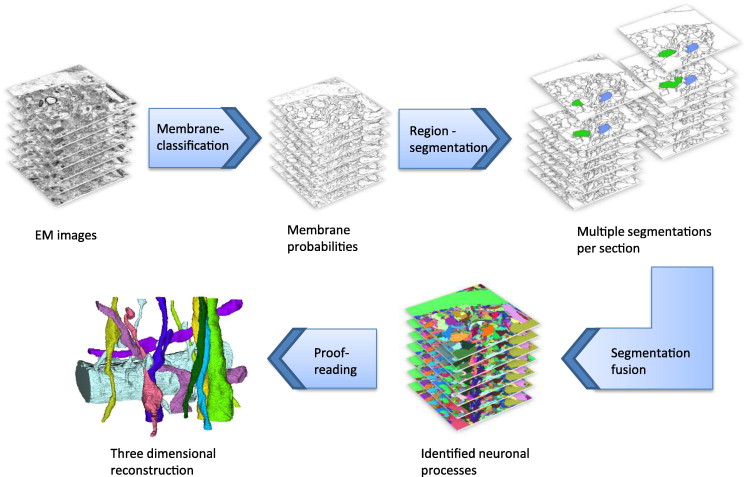
\includegraphics[scale=0.9]{figures/images/reconstruction.jpg}
    \caption[Illustration of a typical workflow for connectome reconstruction]
        {Illustration of a typical workflow for connectome reconstruction.
        Stacks of EM images produced from layers of brain tissue are aligned,
        processed and fused into 3D models that can be studied and simulated.
        Reproduced from \cite{kaynig_large-scale_2015}}
    \label{reconstruction}
\end{figure}
% \vspace{1ex}

A typical workflow for constructing
connectomes is shown in figure \ref{reconstruction}, where large datasets
produced from EM are processed and fused to create a 3D connectome that
re-creates the original observed connectivity, complete with cellular metadata
if enough detail has been resolved. This process is limited by the time and
manual tuning required to process these EM datasets however, as automated
algorithms for processing can produce errors, and the reliability of the
connectome is limited by the quality of the EM data used to create it. 
\autocite{pallotto_extracellular_2015} In
particular, the recognition and reconstruction of network morphology is
especially hard to automate reliably \autocite{helmstaedter_connectomic_2013}.

\subsection[Error induced through noise]{Examination of Error induced through the imaging process}

Prediction of future brain activity through simulation requires an accurate and
detailed connectome of a brain, with synapses and neurons correctly located in
space and the metadata of each neuron in the system replicated with minimal
error \autocite{bostrom_whole_2008}. The accuracy of such a model depends on the
resolution of the imaging method used to create it, and the error resulting from
such a imaging method is the measurement error. Depending on imaging procedure, brain matter may shift in composition during the course of the scan, which is the cause of measurement drift, itself a form of measurement error.

\setlength{\tabcolsep}{4ex}
\renewcommand{\arraystretch}{1.1}
\begin{table}[ht]
    \centering
    \begin{tabular}{@{}llll@{}}
        Method              & Resolution                 & Time    & Error(approx.) \\
        \hline
        MRI                 & 6$\mu m$                   & 30mins  & 95\%           \\
        MRI microscopy      & 3$\mu m$                   & -       & 85\%           \\
        XRay microscopy     & 30nm                       & -       & 30\%           \\
        Electron microscopy & \textasciitilde 30nm-0.1nm & >3mnths & <1\%           \\
        Theoretical Ideal   & <5nm                       & <500s   & <1\%           \\
        \hline
    \end{tabular}
    \DoubleCaption{Comparison of imaging methods.}{Error approximated from size of dendritic spines.}
    \label{imagemethodcomparison1}
\end{table}
\setlength{\tabcolsep}{1ex}

In the above table \ref{imagemethodcomparison1}, I have summarised each of the
major methods that could be considered for imaging the whole human brain. The
theoretical ideal represents the requirements for an imaging process that would
enable the mass creation of connectomes, as a technical requirement of uploading
general human consciousness to vast simulations. These error values will form
the basis of the model and simulation that is described and evaluated later in
this document.

\section{Ethics in Brain Simulation}

\subsection{Ethics in computer science}

% Ethical frameworks that are commonly used in computer science

\subsection{Ethics in related medical research}

% Collecting data
% using data
% Consent and Procedure

\subsection{Ethical considerations for brain simulation}

In "Taking superintelligence seriously: Superintelligence: Paths, dangers,
strategies", Nick Bostrom argues that \ldots \autocite{bostrom_superintelligence_2014}

% Is a brain simulation alive? 
% If accurate enough, how separable is a human and a brain simulation from that human?
% Is it ethical to allow a brain simulation to feel pain? 

% \section{Deductions from this literature review}

% \textsc{TODO Write something here}
